\PassOptionsToPackage{unicode}{hyperref}
\documentclass[aspectratio=1610, professionalfonts, 9pt]{beamer}

\usefonttheme[onlymath]{serif}
\usetheme[showtotalframes]{tudo}

\ifluatex
  \usepackage{polyglossia}
  \setmainlanguage{german}
\else
  \ifxetex
    \usepackage{polyglossia}
    \setmainlanguage{german}
  \else
    \usepackage[german]{babel}
  \fi
\fi


% Mathematik
\usepackage{amsmath}
\usepackage{amssymb}
\usepackage{mathtools}
\usepackage{cancel}

\usepackage{hyperref}
\usepackage{bookmark}
\usepackage{siunitx}

%%%%%%%%%%%%%%%%%%%%%%%%%%%%%%%%%%%%%%%%%%%%%%%%%%%%%%%%%%%%%%%%%%%%%%%%%%%%%%%%
%%%%%-------------Hier Titel/Autor/Grafik/Lehrstuhl eintragen--------------%%%%%
%%%%%%%%%%%%%%%%%%%%%%%%%%%%%%%%%%%%%%%%%%%%%%%%%%%%%%%%%%%%%%%%%%%%%%%%%%%%%%%%

%Titel:
\title{Klassifikation von Erkrankungen der Retina anhand von OCT Bildern}
%Autor
\author[K.~Sedlaczek]{Kevin Sedlaczek, Björn Wendland}
%Lehrstuhl/Fakultät
\institute[Experimental Physics 4/5]{TU Dortmund \\  Physik}
%Titelgrafik
\titlegraphic{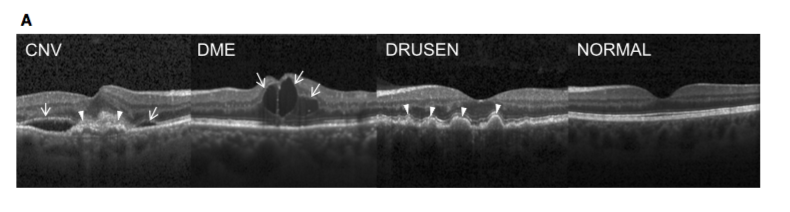
\includegraphics[width=0.95\textwidth]{images/title.png}}


\begin{document}

\maketitle

\begin{frame}{Aufgabenstellung}
  \begin{block}{Fragestellung}
    \centering
    Lässt sich der Zustand einer menschlichen Retina anhand von OCT-Bildern in die 4 Klassen
    %
    \begin{equation*}
        [\text{NORMAL}, \text{CNV}, \text{DRUSEN}, \text{DME}]
    \end{equation*}
    %
    einteilen und somit eine Diagnose mit Hilfe von ML stellen? \\
    \textit{choroidal neovascularization}, \textit{macular edema}, \textit{drusen}
  \end{block}
  \begin{itemize}
    \item \textit{optical coherence tomography}: hoch auflösende Bildgebung von Retina Querschnitten lebender Patienten
    \item Etwa 30 Millionen scans pro Jahr
    \item Analyse durch Mediziner sehr zeitaufwändig
    \item Idee: Automatisierte Methoden um Krankheiten zu erkennen
  \end{itemize}
\end{frame}

\begin{frame}
    \frametitle{Datensatz}
    \begin{itemize}
      \item Inhalt: 84,495 Röntgen Bilder (JPEG) aufgeteilt in 4 Klassen (Erkrankungen + gesund)
      \item Einige Netze bereits trainiert: Genauigkeiten bis \SI{96}{\percent}
    \end{itemize}
    \centering
    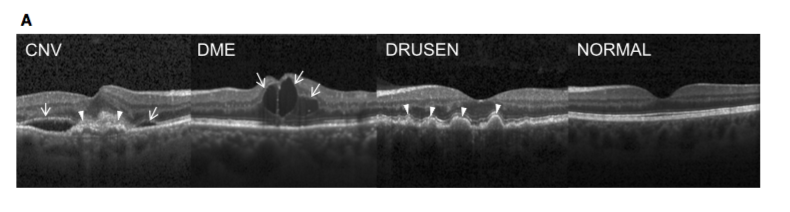
\includegraphics[width=0.8\textwidth]{images/title.png}
\end{frame}

% \begin{frame}
%     \frametitle{Methodik}
%     \begin{itemize}
%       \item Genauigkeit der Diagnosen von Ärzten: 90-\SI{99}{\percent}
%       \item Vergleich mit anderen Modellen:
%       \begin{itemize}
%           \item andere Architekturen
%           \item Modelle auf kleineren subsamples
%       \end{itemize}
%       \item einfache "cut\&count" Methode ohne weitere Parameter schwierig
%     \end{itemize}
% \end{frame}
\end{document}
